%!TEX root = ../bdr.tex
\begin{a3paperl}
\chapter[(Довідковий) Приклад великоформатного додатку]{Приклад великоформатного додатку}\label{apdx:a3}

Якщо ілюстративний матеріал для відображення вимагає більшого ніж А4 формату в класі \verb|bdrvntu| передбачені
оточення для інших форматів аркушу в довільній орієнтації. Даний додаток офрмлений на аркуші А3 формату в альбомній орієнтації.
Для креслеників в класі \verb|bdrvntu| передбачено оточення \verb|drawing| для формування стандартних  штампів на стандартних
форматах аркушів (дивись додаток \ref{apdx:ozpsch}).  

\begin{figure}[h]
 \centering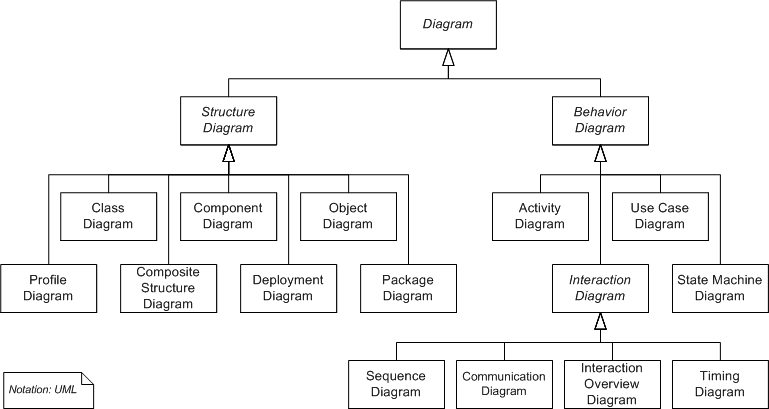
\includegraphics{img/umldiagram.png}
 \caption{UML-діаграма}
 \label{apdxfig:umldiagram}
\end{figure}

\end{a3paperl}

